\chapter{Project Implementation} \label{Project Implementation}

In this section we explore the implementation workflow followed throughout project development phase. This chapter is divided into two main sections, that is, X-rays and CT scans. Within each of these sections, we provide a comprehensive discussion on the approaches and concepts utilized. The implementation workflow ranges from Data Collection to Heatmap Visualization. Before we dive into these sections, we describe our development environment. 

\section{Requirements Analysis}

Our implementation was indeed focused around the Functional Requirements carefully curated during Stage 1 of this project. Most of our requirements revolved around the segmentation and diagnosis of chest X-rays and CT scans, with the former being a mandatory requirement. 

Fortunately, we have been able to experiment with both X-rays and CT scans and successfully build a real-time diagnosis system. Other requirements focused on heatmap generation, multi-class diagnosis, and web interface, which have also been implemented. In addition, we have validated a subset of results obtained with findings observed by a senior Radiologist. 

Our Functional and Non-Functional Requirements generated during Stage 1 along with the Evaluation Strategy can be found in Appendix \ref{Requirements Analysis}.

% We have performed validation of our requirements in Section \ref{reqVal}. 

\section{Development Environment} \label{devEnv}
We have utilized the free-to-use tier of Google Colaboratory to develop our deep learning models. Google provides access to Jupyter Notebooks powered by Tesla K80 GPU with 12 GB RAM and 32 GB disk space. It is also possible for free tier users to access limited number of Tensor Processing Units (TPUs). We have used the latter to enhance performance speed and save processing time.

\section{Source Code}

As mentioned in Section \ref{devEnv}, we have used notebooks provided by Google Colab for developing and evaluating our models. All datasets and notebooks utilized in this project, Flutter code used for our Diagnosis Portal, Python scripts and additional resources are uploaded on our OneDrive repository \footnote{The OneDrive Repository can be found here: \url{https://heriotwatt-my.sharepoint.com/:f:/g/personal/agl2_hw_ac_uk/EmzALshj8olHrfeelAF8h7ABPoVhQBsnViMaiNgTp9Zc6g?e=FbzZhj}}. We have also uploaded the Source Code on GitHub as per the requirements \footnote{GitHub Repository can be found here: \url{https://github.com/AlisterLuiz/Dissertation}}. We have also deployed our Diagnosis Portal that allows real-time COVID-19 Diagnosis \footnote{Link to the Diagnosis Portal: \url{http://40.76.124.61/}}.


\section{X-ray Scans}
The following section illustrates the workflow utilized to collect data, develop and test our deep learning models. We also demonstrate various concepts used to improve model performance.

\subsection{Data Collection}

Our model was trained and tested using images from a Kaggle dataset\footnote{Available at: \url{https://www.kaggle.com/prashant268/chest-xray-covid19-pneumonia}}. The dataset is compiled from multiple  sources \cite{GAN2020, MOO2018, AGC2020}. It is an open-source database of COVID-19 cases which includes X-ray scans. It includes COVID-19 and Pneumonia cases as well as Healthy Chest Scans.


Furthermore, given the objective of our classification task to identify COVID-19 patterns, only the posterior-anterior view of the lungs was considered for training and testing. This view visualizes the bony thoracic cavity, mediastinum, and great vessels \cite{MUR2020}. This choice allowed us to reduce the number of training instances and work with a less unbalanced dataset. 

\subsection{Data Pre-processing}

As we successfully identified a suitable dataset and collected the required X-ray scans, it was now time to pre-process the data and prepare it for model training purposes. This section highlights all the pre-processing procedures we have carried out.

\subsubsection{Data Augmentation} \label{aug}

To generate more training samples and reliable training results we have performed Data Augmentation. It was indeed necessary to balance the dataset before augmenting our scans. 

In each fold of the 10-fold cross validation, we take 10\% of dataset out to be used as validation dataset. The remaining 90\% undergoes an augmentation step. The augmentation step uses three operators to produce slightly modified image, namely rotation, zooming and shearing. Image rotation rotates image by $5^{\circ}$. Zooming applies a +2\% zoom. Shearing distorts an image along an axis (essentially converting rectangles into parallelograms), applies a $2^{\circ}$ counter-clockwise distortion. 

To perform augmentation with these three operators we have utilized Keras' Image Data Generator class which generates batches of tensor image data with real-time data augmentation \cite{KER}. Given memory limits of Google Colab, we have generated 600 images per class using training data which was appended to our existing dataset. Therefore, augmented training data was fed into our deep learning model for training. A summary of our dataset is provided in Section \ref{eda}.

\subsubsection{Exploratory Data Analysis} \label{eda}
As an initial insight into our dataset, we have plotted the number of X-ray scans per class before and after we have balanced the dataset, these figures are plotted in Figure \ref{fig:dataset_dist}. From our initial data collection, we received 575 COVID-19, 4273 Pneumonia, and 2583 healthy chest scans. After balancing, our dataset comprised of 572 scans from each class respectively.

% \vspace{1em}

\begin{figure}[H]
        \begin{subfigure}[b]{0.5\textwidth}
                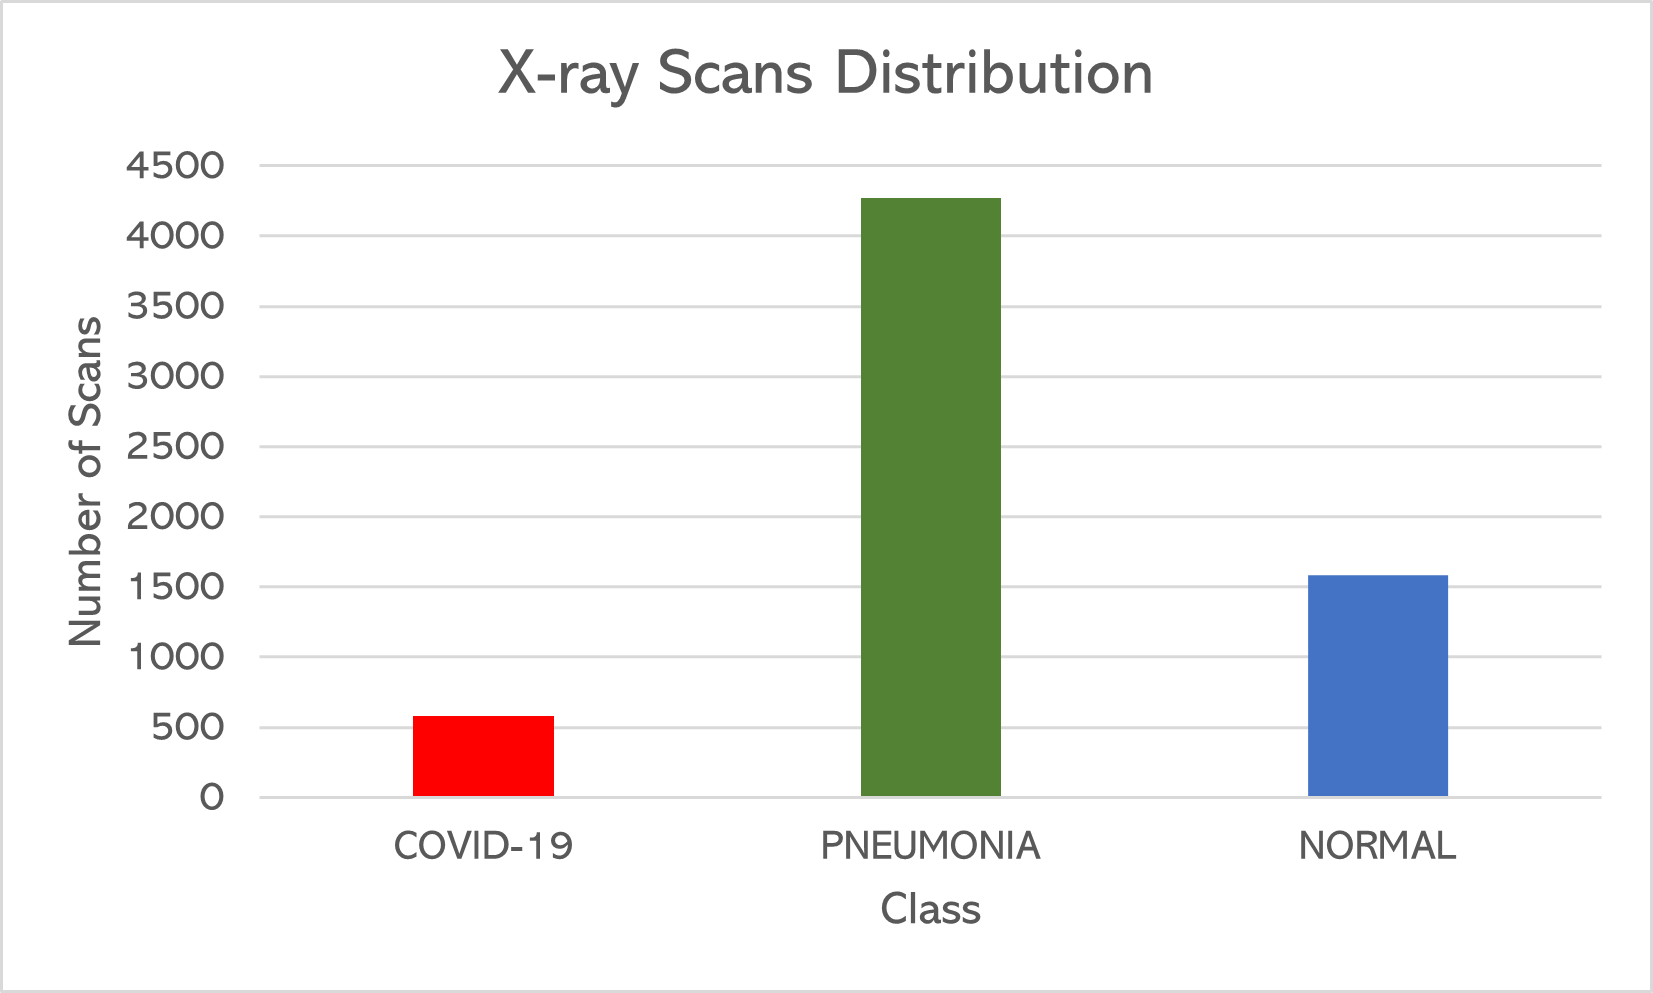
\includegraphics[width=\linewidth]{Images/DatasetDistribution.png}
                \caption{Unbalanced Dataset}
                \label{fig:unbalanced}
        \end{subfigure}%
        \begin{subfigure}[b]{0.5\textwidth}
                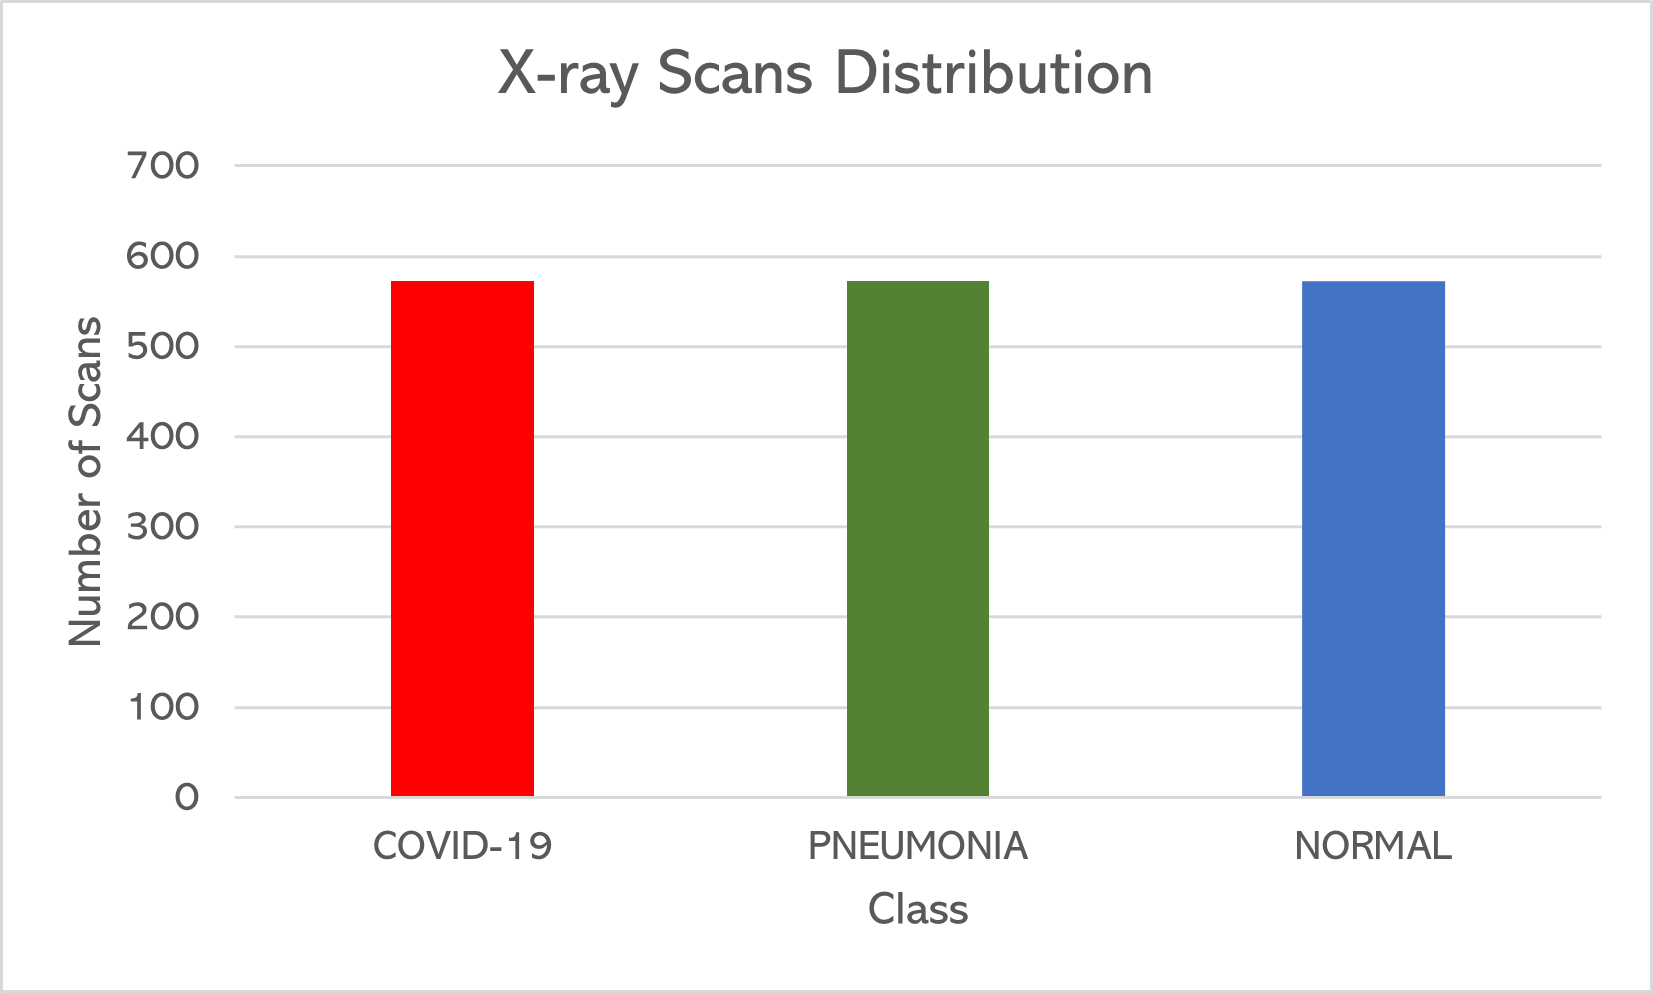
\includegraphics[width=\linewidth]{Images/DatasetDistribution2.png}
                \caption{Balanced Dataset}
                \label{fig:balanced}
        \end{subfigure}%
        %\\\centering
            %\decoRule
        \caption{Dataset Distribution for X-ray Scans}\label{fig:dataset_dist}
\end{figure}
\vspace{-1em}
Post augmentation we have been able to yield more scans per class to further enhance the generalizability of classification. Table \ref{tab:Dataset Info} provides a detailed overview before and after augmentation. Figure \ref{fig:xray data} contains sample X-ray scans from our dataset along with their corresponding labels.

\begin{longtable}{| p{.13\textwidth} | p{.06\textwidth} | p{.18\textwidth} | p{.15\textwidth} | p{.18\textwidth} | p{.11\textwidth} |} 

    \hline
\textbf{Disease} & \textbf{Total}    & \textbf{Non-augmented Training}   &\textbf{Augmented Training} \\
\hline
			COVID-19    &572   &468    &1070
\\\hline
			Pneumonia   &572   &468    &1070
\\\hline
			Normal      &572   &468    &1070
\\\hline 

\caption{Training Dataset Post Augmentation}

  \label{tab:Dataset Info}
    \end{longtable}

\begin{figure}[H]
	\centering
	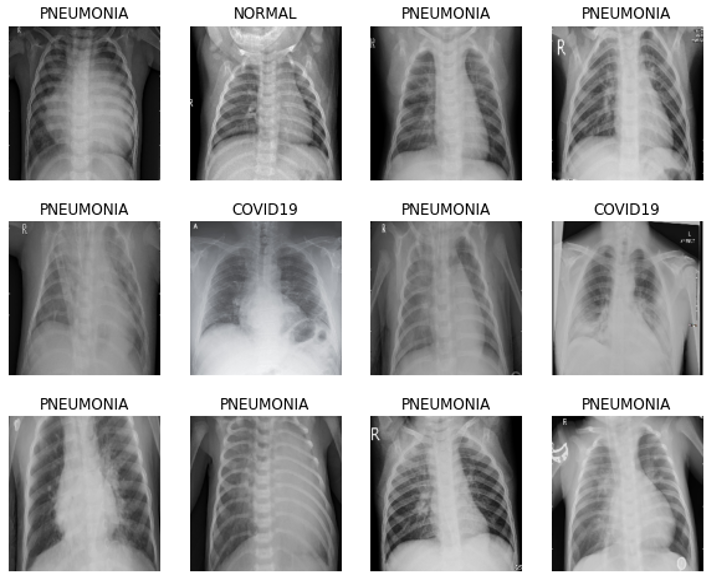
\includegraphics[width=12cm, height=8.5cm]{Images/SampleScans.png}
	
            %\decoRule
	\caption{\small Sample of X-ray scans with labels for model training.}
	\label{fig:xray data}
\end{figure}

\subsection{Methodology}

As we have now explored our dataset, we present the methodology used to construct and develop our deep learning models.  


\subsubsection{Proposed Models}

We have constructed, developed, and evaluated three pre-trained base models on the ImageNet dataset \cite{IMG}, that is, DenseNet121, ResNet50, and VGG16. Each of these base models were trained on the augmented dataset, and ensembled to further improve classification performance. The model architectures for each of these three models are provided in Figure \ref{fig:arch}.

Each of the pre-trained models we have experimented with has their own set of advantages. Dense-Net's are known to ease vanishing-gradient problem, reinforce feature propagation, promote feature reuse, and reduce the number of training parameters \cite{HLW+2016}.

Residual Networks are known for their faster training speeds and powerful representational ability \cite{BAK2016, FEN2017}. Furthermore, from Literature Review (Section \ref{LR}) we observe that ResNet variants seem to be a popular choice among studies performing image classification.
\vspace{0.5em}
\begin{figure}[H]
        \begin{subfigure}[]{0.49\linewidth}
                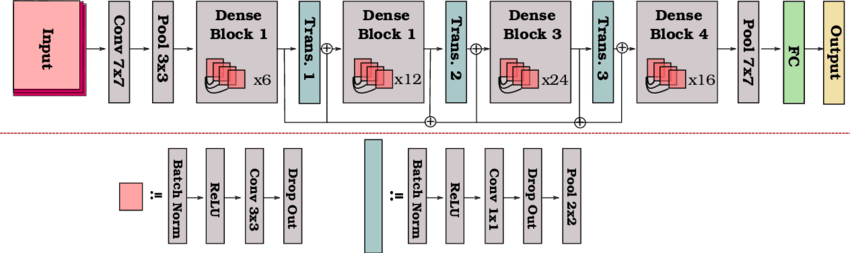
\includegraphics[height=3cm]{Images/DenseNet121.png}
                \caption{DenseNet121 \cite{DEN}}
                \label{fig:DenseNet}
        \end{subfigure}%
        \begin{subfigure}[]{0.49\linewidth}
                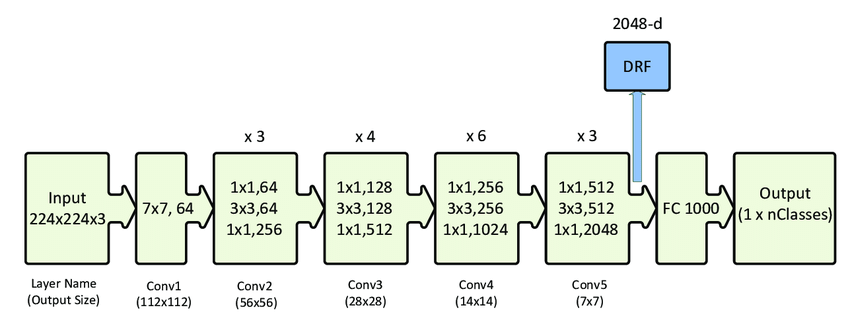
\includegraphics[height=3cm]{Images/ResNet.png}
                \caption{ResNet50 \cite{MOB+2020}}
                \label{fig:ResNet}
        \end{subfigure}%

\end{figure}

\begin{figure}[H]\ContinuedFloat
          \begin{center}
        \begin{subfigure}[]{0.7\linewidth}
                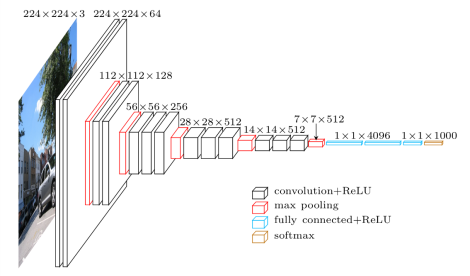
\includegraphics[height=6cm, width=\linewidth]{Images/VGG16.png}
                \caption{VGG16 \cite{VGG}}
                \label{fig:VGG}
        \end{subfigure}%
    
        \end{center}
        %\\\centering
            %\decoRule
        \caption{X-ray Model Architectures}\label{fig:arch}


\end{figure}
\vspace{-2em}
VGG is the simplest model among the three and is usually used for benchmarking \cite{SKZ2015}. Built as a deep CNN, VGG outperforms baselines on many tasks and datasets outside of ImageNet \cite{WJY2019}.

These pre-trained models were readily available on the Keras applications library \cite{KAP}. We have used these pre-trained models as a starting point to build our classification models.

\vspace{1em}

\begin{lstlisting}
pretrainedDenseNet = tf.keras.applications.DenseNet121(input_shape = (imageSize, imageSize, 3), weights = 'imagenet', include_top = False)

pretrainedResNet = tf.keras.applications.ResNet50(input_shape = (imageSize, imageSize, 3), weights = 'imagenet', include_top = False)
pretrainedVGG = tf.keras.applications.VGG16(input_shape = (imageSize, imageSize, 3), weights = 'imagenet', include_top = False)
\end{lstlisting}



\subsubsection{Keras Callbacks} \label{KCXray}

The Keras Callbacks API is an effective utility which aids in enhancing model training. A callback is an object that can perform actions at various stages of training, usually in between epochs or when training begins or ends \cite{KCB}. For training our deep learning models on X-ray scans we utilized three Callback functions, that is, EarlyStopping, ReduceLROnPlateau, and ModelCheckpoint.

EarlyStopping (ES) ends training when a monitored metric has stopped improving \cite{KES}. For each of our deep learning models we have used the ES Callback with the following parameters. 

\vspace{1em}
\begin{lstlisting}
esCallback = tf.keras.callbacks.EarlyStopping(monitor='val_loss', patience=15, verbose=1)
\end{lstlisting}

We monitor validation loss and terminate our training as soon as model converges. An added benefit of using this callback is reduced processing time required to train our deep learning models.

The next callback, ReduceLROnPlateau reduces the learning rate when a metric has stopped improving, in our case validation loss. This callback proved to be fruitful while training our deep learning models. Reducing the Learning Rate by a factor of 0.5, helped the models to converge faster and overcome learning plateaus \cite{KLR}. 
\vspace{1em}
\begin{lstlisting}
lrReduce = tf.keras.callbacks.ReduceLROnPlateau(monitor='val_loss', factor=0.5, min_delta=0.0001, patience=8, verbose=1)
\end{lstlisting}

ModelCheckpoint, simply saves the best performing model during training depending on the given parameter \cite{KMC}.
\vspace{1em}

\begin{lstlisting}
mcpSave = ModelCheckpoint('Path to Save Model', save_best_only=True, monitor='val_loss', mode='min')
\end{lstlisting}

Utilizing each of our these three callbacks allowed us to increase the efficiency and performance of our models.

\subsubsection{Transfer Learning} \label{tl}
Transfer learning is a machine-learning technique where a model trained for an application with some dataset is re-used on another dataset. The pre-trained model approach to transfer learning consists of using the source model as a starting point for training the target model. 

In order to reduce training time and improve accuracy, we adopted the pre-trained transfer learning approach. We have used a model trained with large volume of images from the ImageNet dataset for classification tasks \cite{IMG}. Using the pre-trained model, we trained only the final layer so as to alter its weights to suit our dataset. All other layers used fixed weights obtained from the prior training using the ImageNet dataset. A very simple illustration of the Transfer Learning approach is shown in Figure \ref{fig:transfer learning}. 


\begin{figure}[htbp]
	\centering
	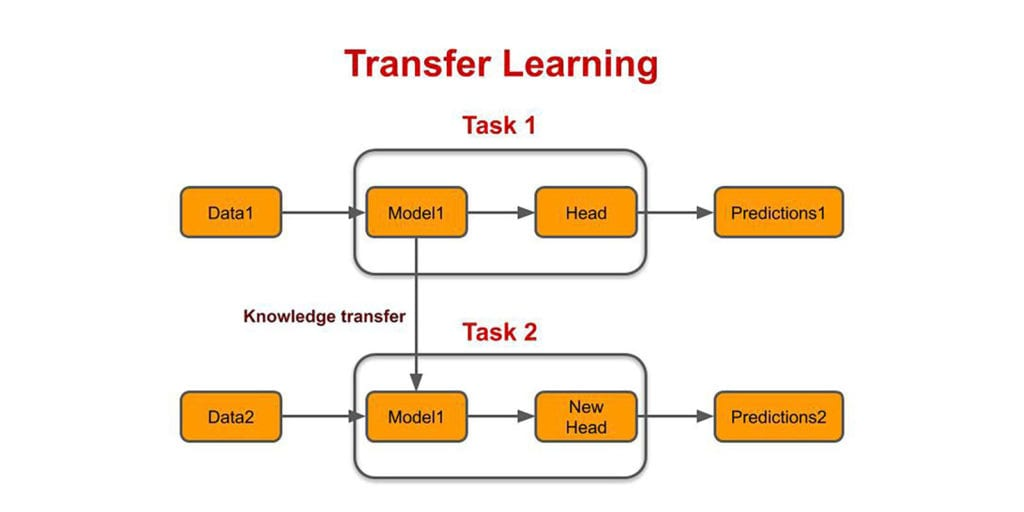
\includegraphics[width=15cm]{Images/Transfer Learning.jpg}
	    %\decoRule
	\caption{\small A simple representation of Transfer Learning Technique \cite{TBT2019}}
	\label{fig:transfer learning}
\end{figure}

\subsubsection{Ensemble Learning} \label{elx}

Given our base models, an ideal approach to improve upon the classification performance was to implement Ensemble Learning. Ensemble Learning involves combining several classifiers to solve a particular problem. The combined model generally achieves optimum predictive performance when compared to any of the constituent learning algorithms alone \cite{POL2019, LUT2017}.

Our approach involves utilizing the best performing model after cross-validation from each of the three base models. We take the last dense layer of each model, that is, without the heads, and provide the network an opportunity to learn from these dense layers before applying the softmax function. Indeed, we have frozen the layer weights of our base models, before ensembling. 

Keras' Concatenate layer \cite{CON} allows us easily merge or stack these dense layers and yield the final prediction after applying the softmax activation. As expected, we have observed an increase in classification performance through ensembling our base models. An illustration of the same is provided in Figure \ref{fig:ensemble learning}.

\begin{figure}[H]
	\centering
	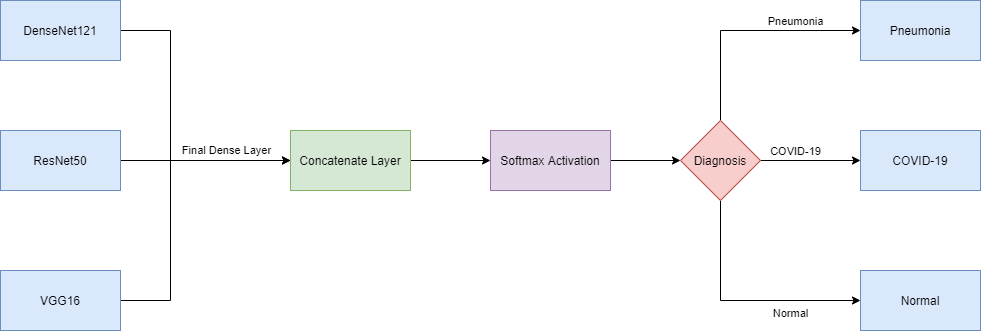
\includegraphics[width=15.5cm]{Images/Ensemble.png}
	    %\decoRule
	\caption{\small Ensemble Learning Illustration for X-ray Scans}
	\label{fig:ensemble learning}
\end{figure}


\subsubsection{Model Training}

We have used 10-fold cross validation and leave an eleventh fold to test the 10 models on it as unseen data. Indeed, 10-fold cross validation produces 10 models that, collectively, saw all the training dataset. We have seen our dataset distribution is Section \ref{eda}. We built a balanced dataset of 572 samples of each of the classes (572 is a multiple of 11). The size of the eleventh fold, to which we refer to from now on as \textit{unseen data}, is 52. 

\begin{longtable}{| p{.13\textwidth} | p{.06\textwidth} | p{.18\textwidth} | p{.15\textwidth} | p{.18\textwidth} | p{.11\textwidth} |} 

    \hline
\textbf{Disease} & \textbf{Total}    & \textbf{Non-augmented Training}   &\textbf{Augmented Training} &\textbf{Non-augmented Testing} & \textbf{Unseen Data} \\
\hline
			COVID-19    &572   &468    &1070   &52   &52
\\\hline
			Pneumonia   &572   &468    &1070   &52   &52
\\\hline
			Normal      &572   &468    &1070   &52   &52
\\\hline 

\caption{Dataset Distribution}

  \label{tab:Dataset Info}
    \end{longtable}
\vspace{-1em}
At each of the 10 iterations of 10-fold cross validation, we take 10\% of the dataset out to be used for testing. The remaining 90\% undergoes the augmentation steps as mentioned in Section \ref{aug}. 

The augmentation of each of the 468 samples of each class (90\% of 520) resulted in creating 1070 samples per class. Since we have three classes, COVID-19, Pneumonia and Normal, the total number of samples in the final training dataset is of 3,210. Only the training dataset was augmented; no augmentation was applied to the test dataset. Table \ref{tab:Dataset Info} shows the size of the data we used. 

We trained our models for 50 epochs with a batch size of 210 per forward/backward pass. We have also initialized all the callbacks mentioned in Section \ref{KCXray}. Post training, the results were evaluated using scikit-learns classification report function \cite{SCR}. A confusion matrix was also displayed after every epoch indicating the model performance \cite{SCM}, which also allows us to extract useful metrics and determine the best performing model. A sample snippet of code which calls the fit function is provided below.

\vspace{1em}
\begin{lstlisting}
history = model.fit(augmentedDataX, YCatAug, validation_data = (XTrain[test], YCatVal), callbacks=[lrReduce, esCallback, mcpSaveDenseNet], epochs=50, batch_size=210)
\end{lstlisting}

\subsubsection{Heatmap Visualization}

For the purpose of building a more interepretable model, we generated heatmaps for the provided X-ray scans. The heatmaps highlight the regions that led to the classification by our model. We calculated the Grad-CAM heatmaps with the help of Keras' Computer Vision examples \cite{KCV}. The same Grad-CAM class activation visualization example provided by François Chollet was utilized in our implementation \cite{KGM}. We have generated Grad-CAM heatmaps from each of our three base models. We have utilized Numpy \cite{NUM} to average obtained heatmaps and produce the final consolidated heatmap.

Grad-CAM heatmaps highlight regions in the lungs which, as discussed in section \ref{Interpreting Deep Learning Results}, exhibit the most common characteristics in patients diagnosed with COVID-19. These include features such as GGO’s, consolidations, lesions, and crazy-paving patterns, which are some of the most contributing features to diagnosis. This technique provides interpretation means that would assist radiologists in identifying the same lung characteristics as with traditional segmentation-based methods. Regions in red are the most influential in making the decision, whereas blue regions are the least influential.


\subsubsection{Workflow Summary Illustration}

\begin{figure}[H]
	\centering
	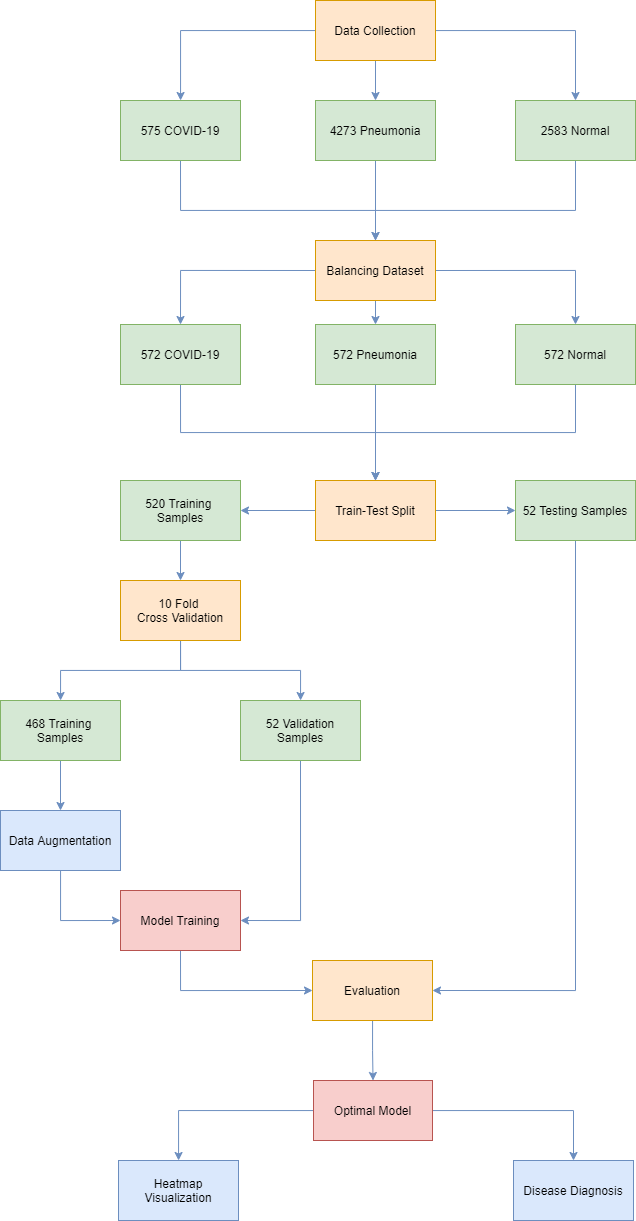
\includegraphics[width=13cm, height= 22.5cm]{Images/X-ray Workflow.png}
	    %\decoRule
	\caption{\small X-ray Workflow Illustration}
	\label{fig:Xray Illustration}
\end{figure}

\section{CT Scans}
The following section explores the second part of our project, that is, CT scans. A similar workflow has been utilized for CT classification purposes with minor changes in between such as Lung Parenchyma extraction as an additional pre-processing step.

\subsection{Data Collection}

We have used an open-source Kaggle CT dataset \footnote{Available at \url{https://www.kaggle.com/azaemon/preprocessed-ct-scans-for-covid19}} for training and testing our models. All the images present in this dataset was collected by the authors from the Frontier Exploration Program of Huazhong University of Science and Technology, the program for HUST Academic Frontier Youth Team, and the Fundamental Research Funds for the Central Universities \cite{JCY+2020, ICT2019}. 

This dataset is comprised of two parts, the original and pre-processed CT scans of COVID-19 and Normal patients readily available for model training purposes. The code to pre-process the original CT scans was given by the author of this dataset. Applying them we were able to extract the lung parenchyma, which proved to be a vital pre-requisite to train CT data.

\subsection{Data Pre-processing}

In the following subsections, we provide a brief overview on the various Data Pre-processing techniques we have applied. 
\subsubsection{Lung Parenchyma Extraction}

Even though the Kaggle dataset already contains the pre-processed dataset, it was necessary for us to understand the process involved in extracting the lung parenchyma, so as to do the same for incoming unseen samples in a real-time application.

This process for extracting the lung parenchyma was as per the suggestions by Ning et al. \cite{ICT2019}. The source code involved a fill water function that applied certain filter masks to further fine tune the extracted lung parenchymas. An example of a CT scan image before and after extracting lung parenchyma is displayed in Figure \ref{fig:extract}. Indeed, the processed CT images were used for model training and evaluation purposes.

\begin{figure}[H]
        \begin{subfigure}[b]{0.5\textwidth}
                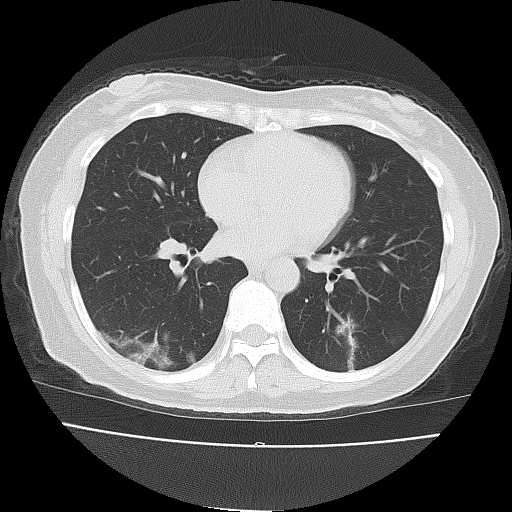
\includegraphics[width=\linewidth]{Images/NonProcessed pCT1.jpg}
                \caption{Original CT Scan}
                \label{fig:unbalanced}
        \end{subfigure}%
        \begin{subfigure}[b]{0.5\textwidth}
                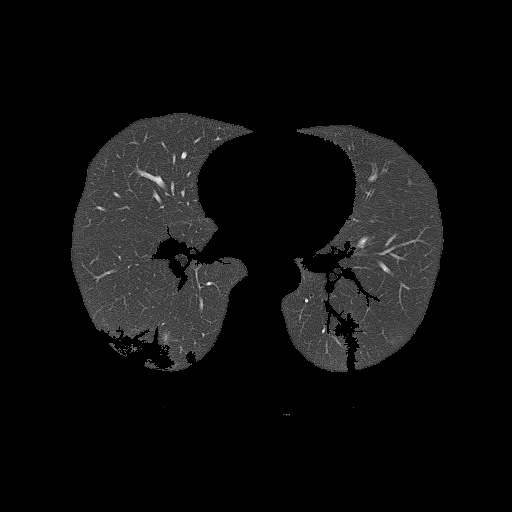
\includegraphics[width=\linewidth]{Images/Processed pCT1.jpg}
                \caption{Processed CT Scan}
                \label{fig:balanced}
        \end{subfigure}%
        %\\\centering
            %\decoRule
        \caption{Lung Parenchyma Extraction}\label{fig:extract}
\end{figure}

\subsubsection{Data Augmentation}

Similar to our X-ray pre-processing workflow we have augmented the CT data so as to improve the reliability of our model prediction and handle unpredictabilities of real-world data. The same augmentation parameters were applied at each of the 10 iterations of 10-fold cross validation, that is, $5^{\circ}$ rotation, +2\% zooming, and $2^{\circ}$ shearing. Keras' Image Data Generator class was once again utilized for performing real-time data augmentation \cite{KER}. Once again prioritizing the limits of Google Colab, we have generated 2000 augmented images per class and is appended to the existing dataset.

\subsubsection{Exploratory Data Analysis} \label{EDA CT}

To familiarize ourselves with the data, the first step was to plot the number of CT scans per class. Similar to X-ray scans, the plots include the counts before and after balancing the dataset. The plots are displayed in Figure \ref{fig:CTdist}. The number of training scans post augmentation is tabulated in Table \ref{tab:Dataset Info CT}. After collecting data from the Kaggle Dataset we have ended up 4001 COVID-19 and 9979 Normal scans. After balancing our dataset we have ended up with 3993 scans per class.

\begin{figure}[H]
        \begin{subfigure}[b]{0.5\textwidth}
                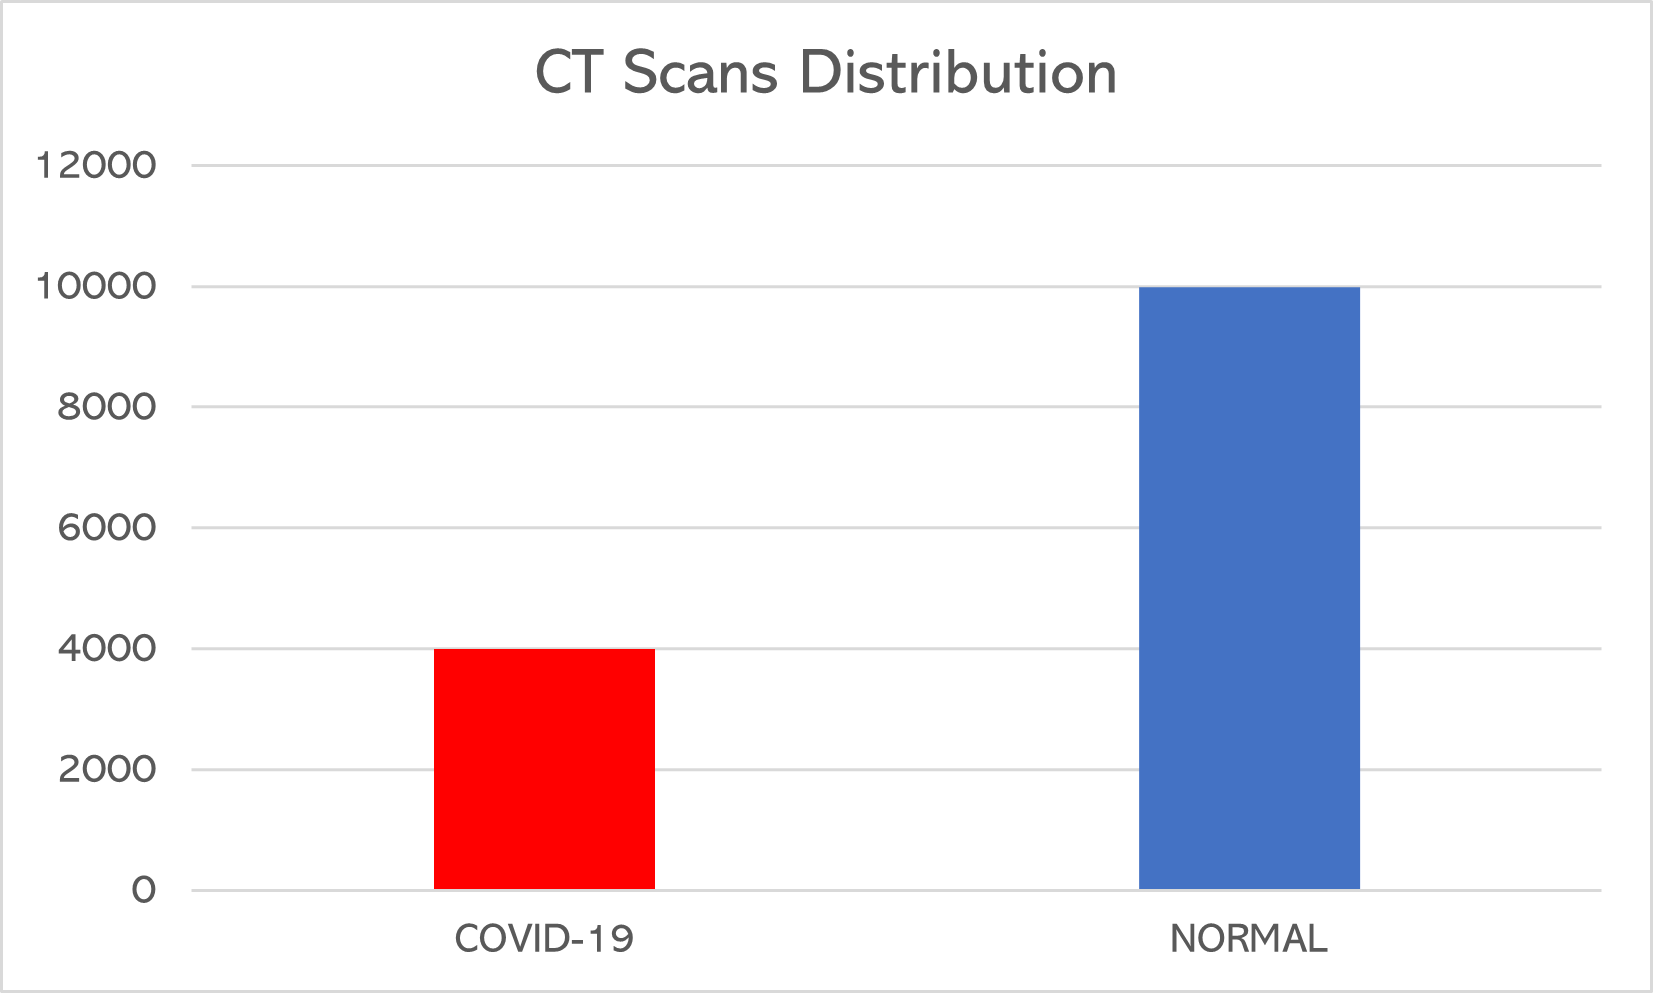
\includegraphics[width=\linewidth]{Images/CTDistribution.png}
                \caption{Unbalanced Dataset}
                \label{fig:unbalanced}
        \end{subfigure}%
        \begin{subfigure}[b]{0.5\textwidth}
                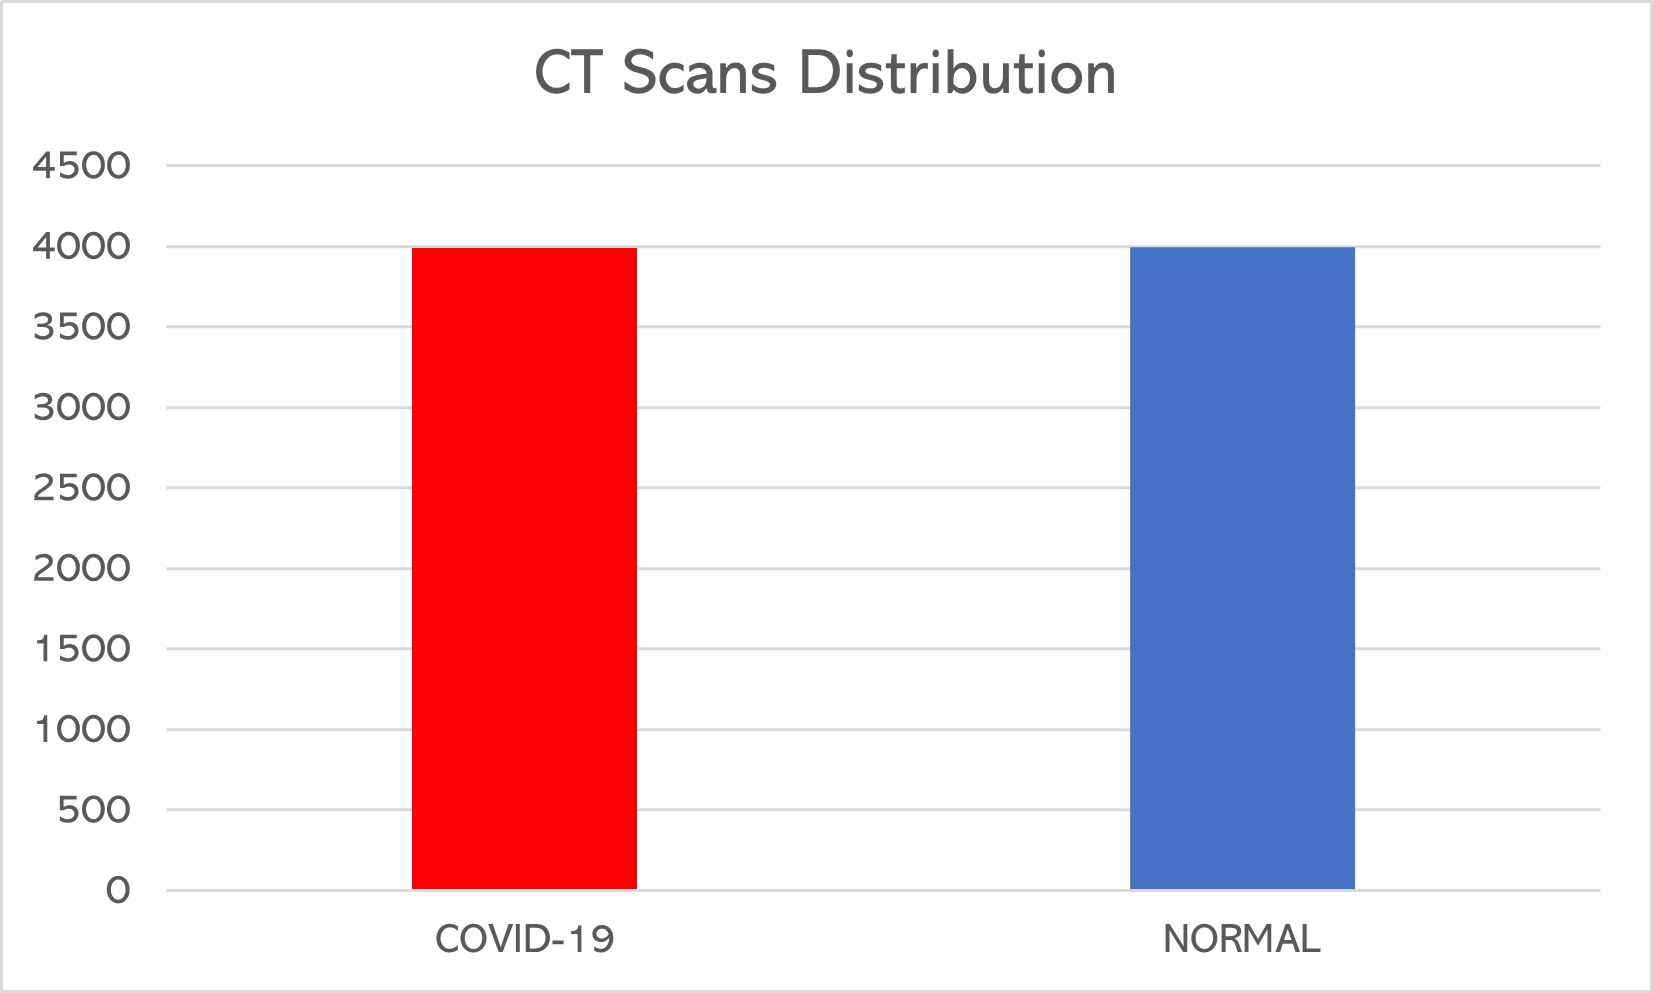
\includegraphics[width=\linewidth]{Images/CTDistribution2.png}
                \caption{Balanced Dataset}
                \label{fig:balanced}
        \end{subfigure}%
        %\\\centering
            %\decoRule
        \caption{Dataset Distribution}\label{fig:CTdist}
\end{figure}

\begin{longtable}{| p{.13\textwidth} | p{.06\textwidth} | p{.18\textwidth} | p{.15\textwidth} | p{.18\textwidth} | p{.11\textwidth} |} 

    \hline
\textbf{Disease} & \textbf{Total}    & \textbf{Non-augmented Training}   &\textbf{Augmented Training} \\
\hline
			COVID-19    &3993   &3267    &5270
\\\hline
			Normal      &3993   &3267    &5270
\\\hline 

\caption{Training Dataset Post Augmentation}

  \label{tab:Dataset Info CT}
    \end{longtable}

We have also displayed a subset of our CT scans dataset along with their labels in Figure \ref{fig:ct data}.


\begin{figure}[H]
	\centering
	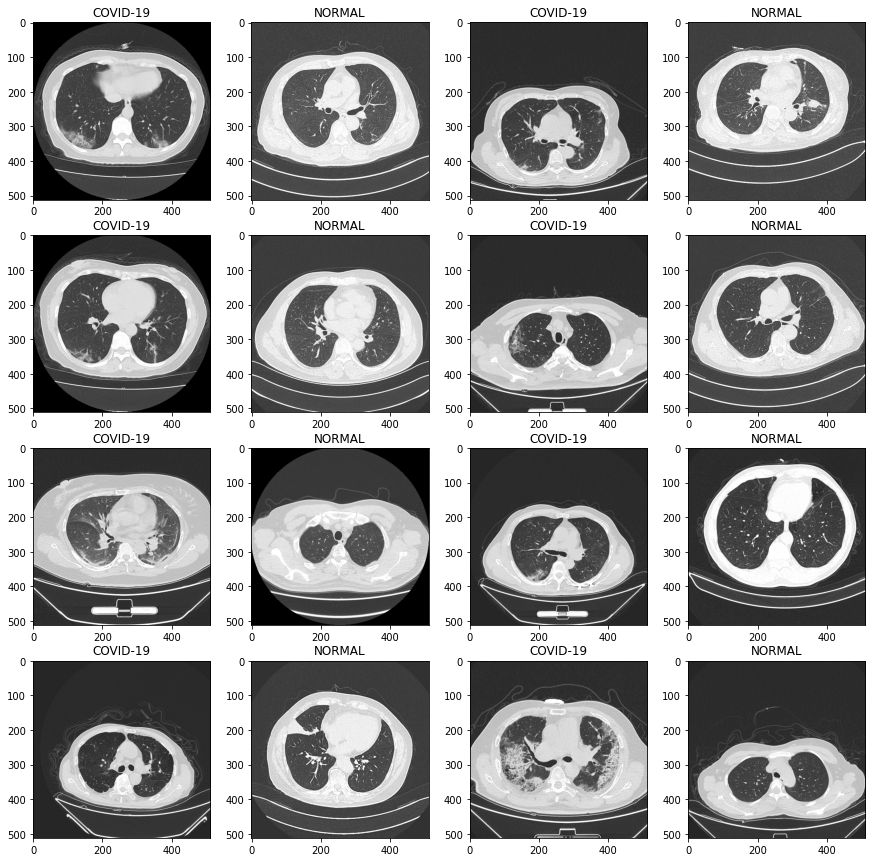
\includegraphics[width=10.5cm, height=10.5cm]{Images/CTScansDist.png}
            %\decoRule
	\caption{\small Sample of unprocessed CT scans with labels for model training.}
	\label{fig:ct data}
\end{figure}

\subsection{Methodology}

Our proposed methodology for CT scans is similar to that of X-ray's to keep our workflow consistent. There are indeed changes in our proposed models and certain parameter values. The following sections elaborates on these differences. 
\subsubsection{Proposed Models}

For CT Scans we have experimented with three models, that is, UNet, UNet++, and Attention UNet. These variants of the base UNet model seems to be popular among literature. The UNet++ and Attention UNet models were Ensembled to improve the classification performance, similar to our X-ray diagnosis workflow. Each of these three model architectures are provided in Figure \ref{fig:ctmodels}.

The UNet model was originally created for Bio-medical Image Segmentation purposes \cite{RFT2015}. As its name indicates, the architecture consists of a 'U' structure, as shown in Figure \ref{fig:unet}. The basic idea revolves around the notion that the same feature maps used for image contraction is utilized to expand a vector to a segmented image. This would help in preserving the structural integrity of the image and greatly reduce image distortion \cite{HSA2018}. The UNet architecture is comprised of three sections, which are, contraction, bottleneck, and expansion respectively.

\begin{figure}[H]
        \begin{subfigure}[b]{0.5\textwidth}
                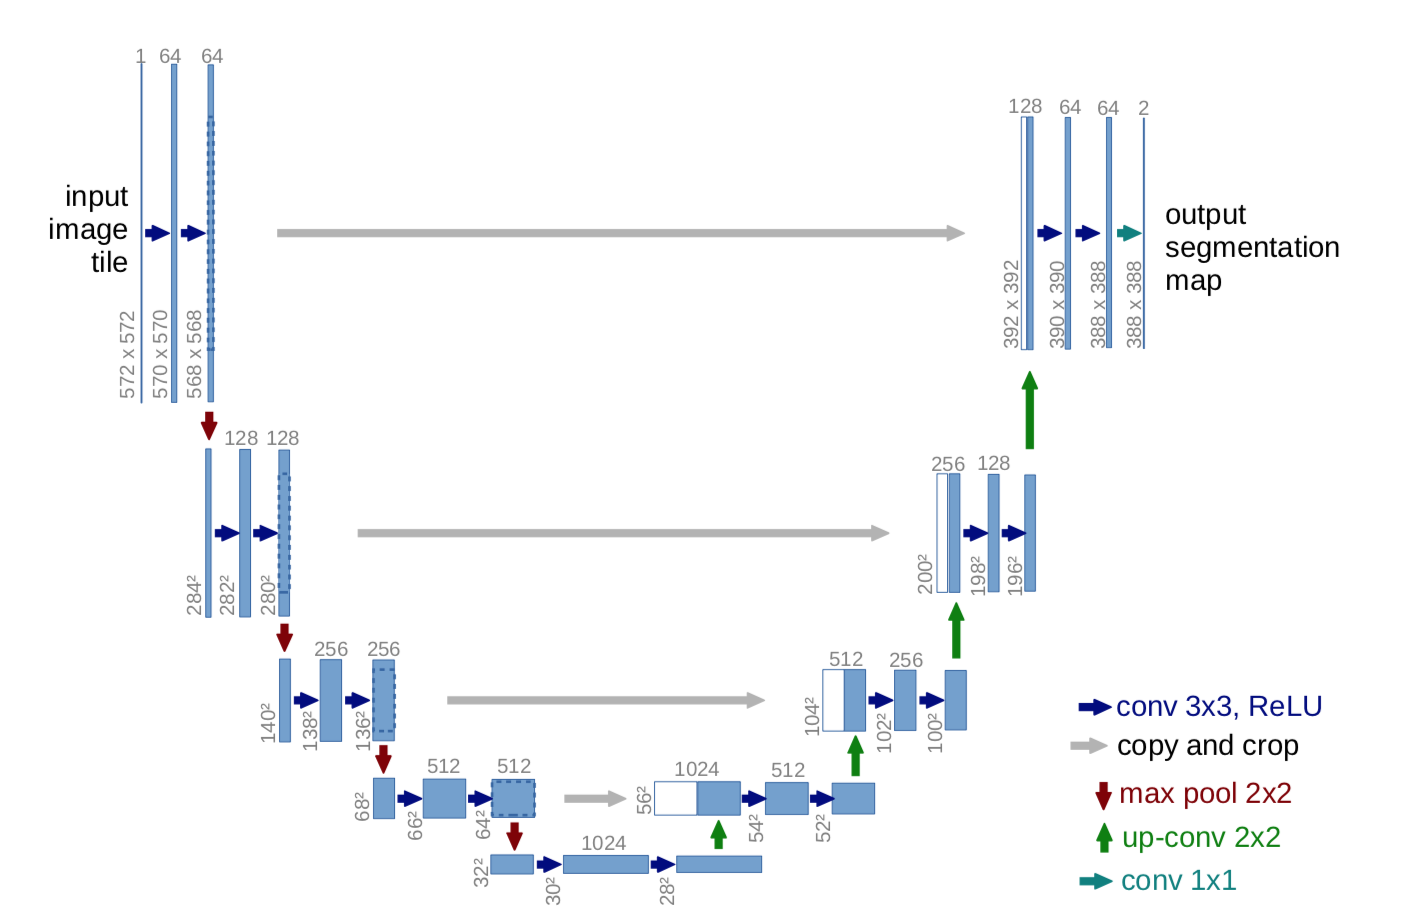
\includegraphics[height=4cm]{Images/UNet.png}
                \caption{UNet \cite{UNT}}
                \label{fig:unet}
        \end{subfigure}%
        \begin{subfigure}[b]{0.5\textwidth}
                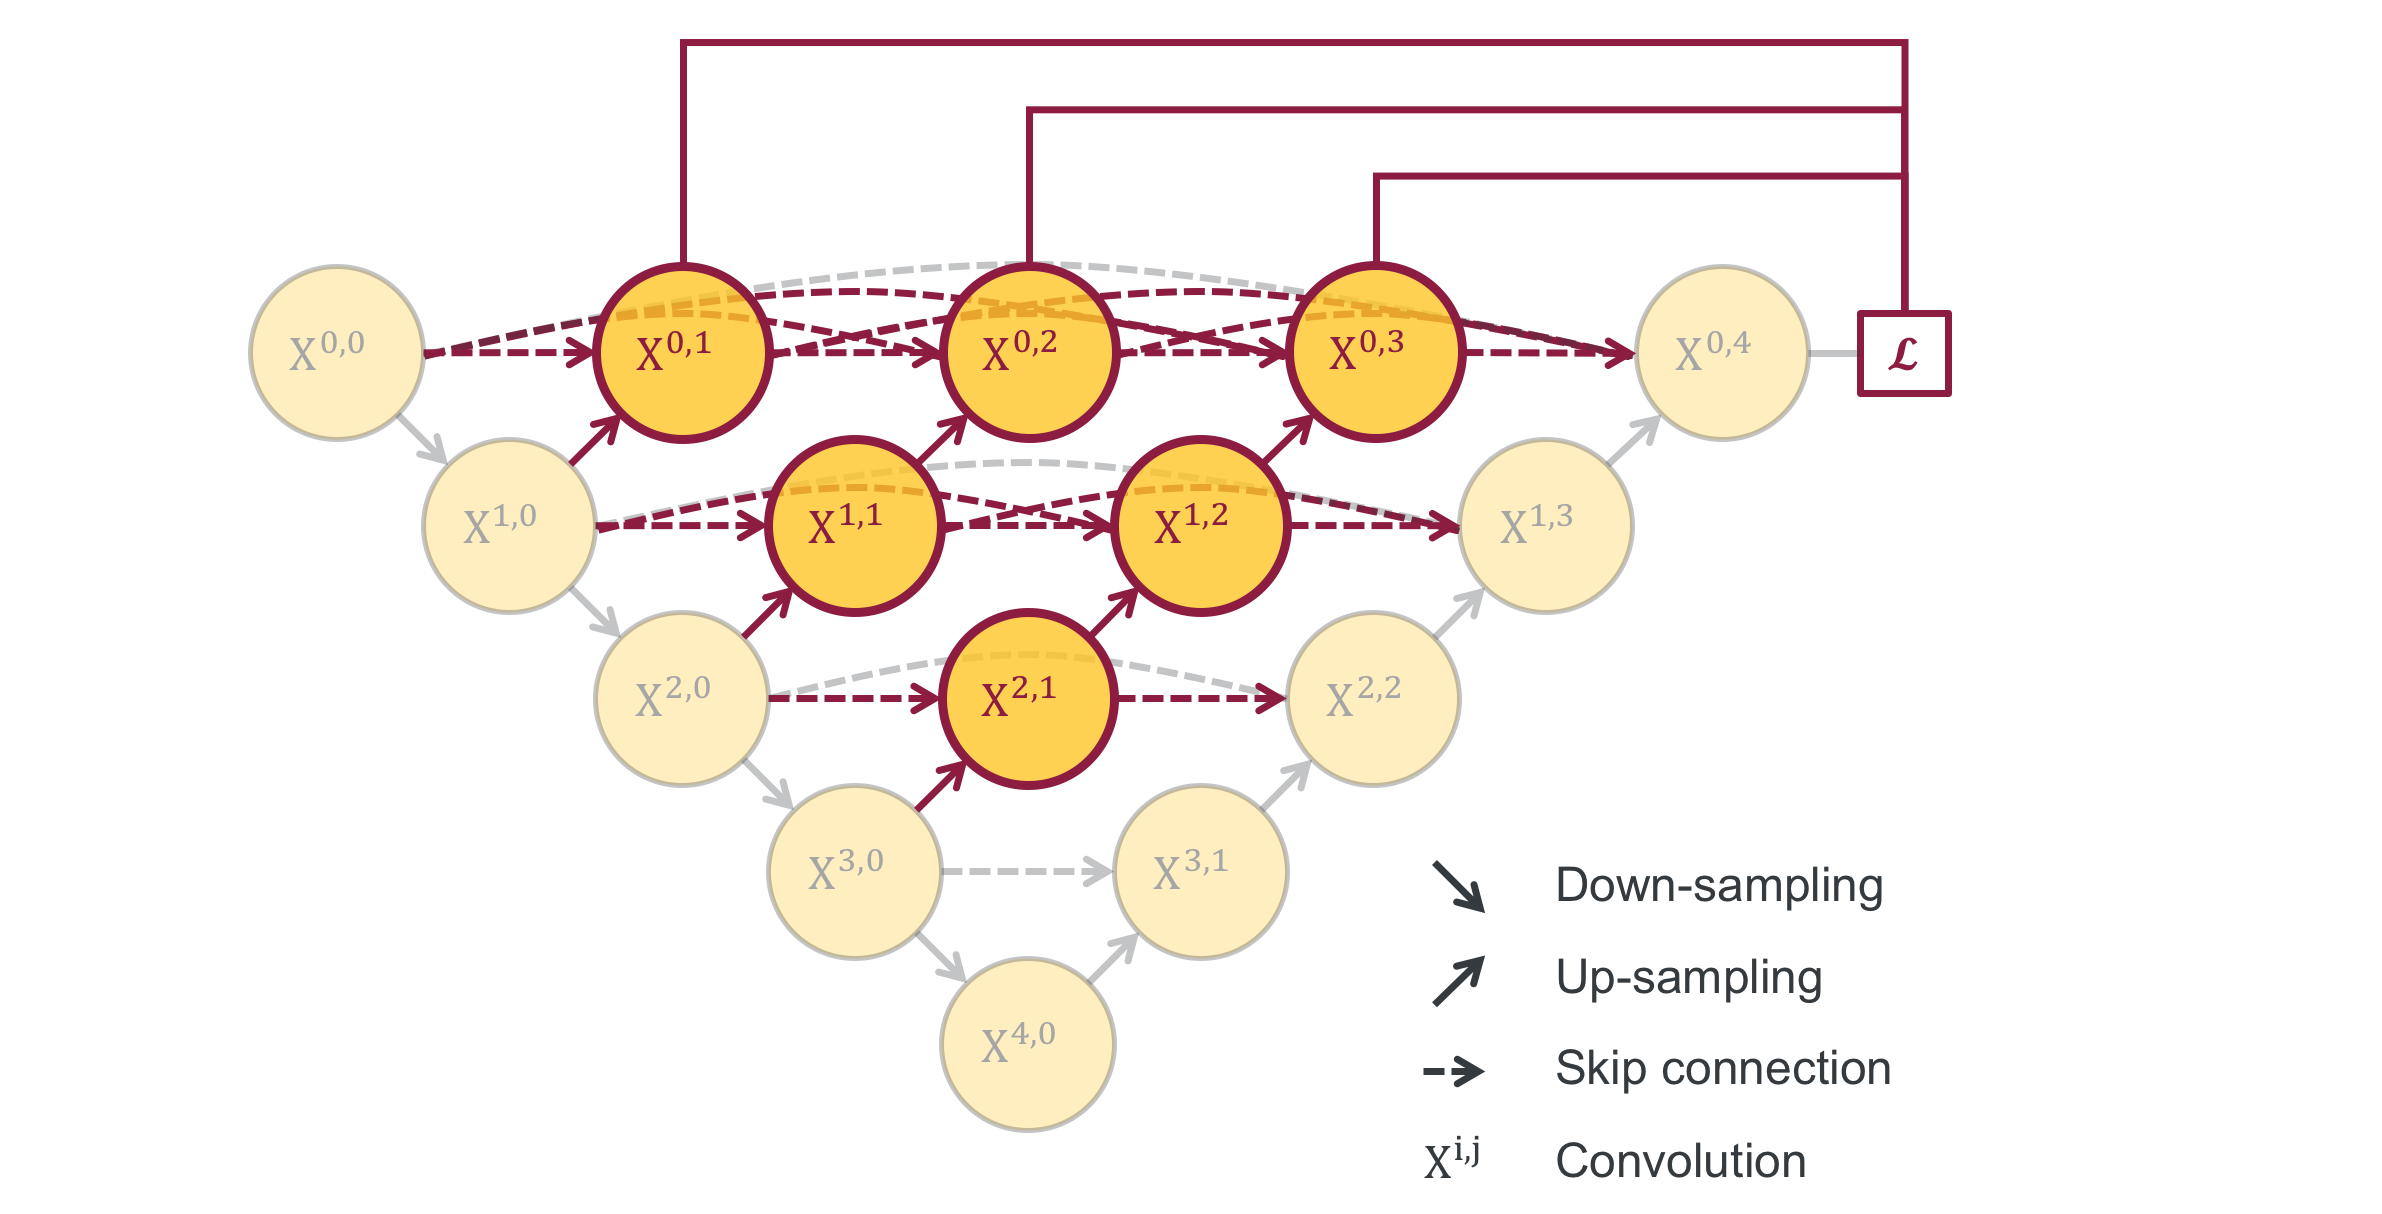
\includegraphics[height=4cm]{Images/UNet++.png}
                \caption{UNet++ \cite{UNT+}}
                \label{fig:unet++}
        \end{subfigure}\\\\
        \begin{center}
         \begin{subfigure}[b]{0.5\textwidth}
                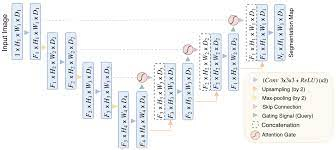
\includegraphics[width=\linewidth]{Images/Att UNet.jpg}
                \caption{Attention UNet \cite{AUN}}
                \label{fig:attUnet}
        \end{subfigure}%
        %\\\centering
            %\decoRule
        \caption{CT Model Architectures}\label{fig:ctmodels}
        \end{center}
\end{figure}

UNet++ is another powerful architecture for medical image segmentation \cite{ZSM+2020}. UNet++ has three major additions when compared to the original UNet model proposed by Ronneberger, that is, redesigned skip pathways, dense skip connections, and deep supervision \cite{JHJ2019}. One caveat of using the UNet++ due to these additions is that the training time is almost doubled when compared to a simple UNet.

Attention UNet aims to only highlight the relevant activations during training, thus significantly reducing computation time. This is made possible using attention gates which uses additive soft attention. As its name suggests, the name pays attention or focuses on certain parts of the provided image \cite{VIN2020, OSF+2020}. When compared to a UNet model, the computation time is only slightly longer. The code snippets initializing each of the three models have been provided below.

\vspace{1em}
\begin{lstlisting}
pretrainedUNet = kerasModels.unet_2d((imageSize, imageSize, 3), filter_num=[64, 128, 256, 512, 1024], n_labels=2, stack_num_down=2, stack_num_up=2, activation='ReLU', output_activation='Sigmoid', batch_norm=True, pool=False, unpool=False, backbone='ResNet50V2', weights='imagenet', freeze_backbone=True, freeze_batch_norm=True, name='unet') 

pretrainedUNetPlus = kerasModels.unet_plus_2d((imageSize, imageSize, 3), filter_num=[64, 128, 256, 512, 1024], n_labels=2, stack_num_down=2, stack_num_up=2, activation='ReLU', output_activation='Sigmoid', batch_norm=True, pool=False, unpool=False, backbone='ResNet50V2', weights='imagenet', freeze_backbone=True, freeze_batch_norm=True, name='unetplus')

pretrainedAttUNet = kerasModels.att_unet_2d((imageSize, imageSize, 3), filter_num=[64, 128, 256, 512, 1024], n_labels=2, stack_num_down=2, stack_num_up=2, activation='ReLU', atten_activation='ReLU', attention='add', output_activation='Sigmoid', batch_norm=True, pool=False, unpool=False, backbone='ResNet50V2', weights='imagenet', freeze_backbone=True, freeze_batch_norm=True,  name='attunet') 
\end{lstlisting}

\subsubsection{Keras Callbacks}

We have utilized the same set of callbacks as we have used for our X-ray models, that is, EarlyStopping, ReduceLROnPlateau, and ModelCheckpoint. However, there have been differences in the parameters especially for EarlyStopping as the UNet models tend to stop training before reaching convergence. Therefore, it was necessary for us to increase the patience parameter depending the variant of UNet model. The following code snippets showcase the parameters used for EarlyStopping Keras callback.

\vspace{1em}
\begin{lstlisting}
UNetESCallback = tf.keras.callbacks.EarlyStopping(monitor='val_loss', patience=80, verbose=1)
AttUNetESCallback = tf.keras.callbacks.EarlyStopping(monitor='val_loss', patience=80, verbose=1)
UNetPlusESCallback = tf.keras.callbacks.EarlyStopping(monitor='val_loss', patience=140, verbose=1)
\end{lstlisting}

Furthermore, for the UNet++ model we have provided custom parameters for the ReduceLROnPlateau callback to achieve optimal convergence and thereby increase classification accuracy.

\vspace{1em}
\begin{lstlisting}
UNetPluslrReduce = tf.keras.callbacks.ReduceLROnPlateau(monitor='val_loss', factor=0.5, min_delta=0.0001, patience=16, verbose=1)
\end{lstlisting}

\subsubsection{Transfer Learning}

We have applied the Transfer Learning technique for CT scan classification as well to avail its benefits such has reduced training time and improvement in accuracy as discussed in Section \ref{tl}. The only difference from our X-ray scan implementation is that we have used a different Python package, Keras UNet Collection \cite{KUC}, which contains pre-trained UNet model and its variants on the large ImageNet dataset \cite{IMG}. 

This package allowed us to easily access different UNet variants and contains various tweakable parameters allowing us to customize or fine-tune our models for training and evaluation purposes. From the code snippet we can clearly see the weights parameter which initializes the model with ImageNet weights. Similar to our X-ray implementation, we have only set the final layer to be trainable.

\vspace{1em}
\begin{lstlisting}
pretrainedUNet = kerasModels.unet_2d((imageSize, imageSize, 3), filter_num=[64, 128, 256, 512, 1024], n_labels=2, stack_num_down=2, stack_num_up=2, activation='ReLU', output_activation='Sigmoid', batch_norm=True, pool=False, unpool=False, backbone='ResNet50V2', weights='imagenet', freeze_backbone=True, freeze_batch_norm=True, name='unet') 
\end{lstlisting}

\subsubsection{Ensemble Learning}

We have ensembled the UNet, Attention UNet and UNet++ models to further boost our classification performance on the CT dataset. We have utilized a similar ensembling workflow but with different base models as discussed in Section \ref{elx}. We have extracted the final dense layer, froze all the trained layers from each of our base models to prevent re-training, and simply merged these dense layers before applying the softmax function. Once again, through ensembling we have observed an increase in model classification performance. Figure \ref{fig:ct ensemble} displays an illustration of our ensemble learning workflow for CT scans.

\begin{figure}[H]
	\centering
	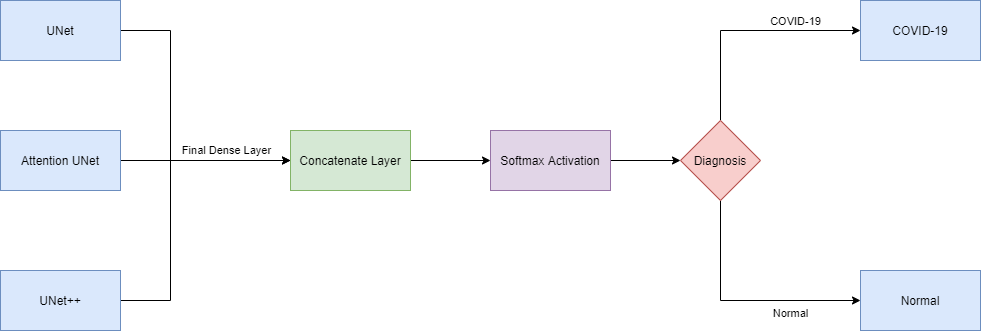
\includegraphics[width=15.5cm]{Images/EnsembleCT.png}
            %\decoRule
	\caption{\small Ensemble Learning Illustration for CT Scans}
	\label{fig:ct ensemble}
\end{figure}

\subsubsection{Model Training}

We have once again utilized 10-fold cross validation to train our CT models. We have also left an eleventh fold to test our model on unseen data. As seen from Section \ref{EDA CT}, we have built a balanced dataset comprised of 3993 samples from each class (3993 is a multiple of 11). The size of the eleventh fold also referred to as \textit{unseen data}, is 363.

At each iteration of the 10-fold cross validation, 90\% of the training data undergoes the augmentation steps and the remaining 10\% is used for validation purposes.

\begin{longtable}{| p{.13\textwidth} | p{.06\textwidth} | p{.18\textwidth} | p{.15\textwidth} | p{.18\textwidth} | p{.11\textwidth} |} 

    \hline
\textbf{Disease} & \textbf{Total}    & \textbf{Non-augmented Training}   &\textbf{Augmented Training} &\textbf{Non-augmented Testing} & \textbf{Unseen Data} \\
\hline
			COVID-19    &3993   &3267    &5270   &363   &363
\\\hline
			Normal      &3993   &3267    &5270   &363   &363
\\\hline 

\caption{Dataset Distribution for CT Scans}

  \label{tab:CT Dataset Info}
    \end{longtable}
\vspace{-1em}

Augmentation of 3267 samples from each class resulted in 5270 samples as our augmented training dataset. Our final training dataset is therefore comprised of 10,540 samples as we have two classes, COVID-19 and Normal. Indeed, only the training dataset was augmented, our testing dataset was left aside only for validation purposes. Table \ref{tab:CT Dataset Info} displays the size of our data.

We have trained our UNet and Attention UNet models for 200 epochs each, whereas for UNet++ it took around 300 epochs to achieve convergence. The batch size was 1024 samples per forward/backward pass. Our ensemble model was trained for 50 epochs to give it an opportunity to learn from the final dense layers from each of our base models before returning a prediction. Similar to X-ray scans, we have initialized the same callbacks, and returned the classification report \cite{SCR} and confusion matrix \cite{SCM} after every fold which allowed us to determine the best performing model.

% A sample snippet of code is provided below.

% \vspace{1em}
% \begin{lstlisting}
% history = model.fit(augmentedDataX, YCatAug, validation_data = (XTrain[test], YCatVal), callbacks=[ESCallback, lrReduce, mcpSave], epochs=200, batch_size=1024)
% \end{lstlisting}

\subsubsection{Heatmap Visualization}

For interpreting our model's results we have generated heatmaps in addition to the diagnosis result. The same Grad-CAM technique utilizing Keras library \cite{KCV} was applied in the case of CT scans to highlight common characteristics in patients diagnosed with COVID-19. We have once again averaged the heatmaps produced by each of our three base models with the help of Numpy \cite{NUM} to obtain the final heatmap. We believe these heatmaps would aid radiologists in identifying the same lung characteristics more efficiently.

There was only one difference in our implementation when compared to X-rays. Given a test image, it was necessary for us to extract the lung parenchyma before proceeding with the diagnosis and generating the heatmaps. The heatmap filter generated was superimposed to our unprocessed CT input in order to highlight the most critical regions.

\subsubsection{Workflow Summary Illustration}

\begin{figure}[H]
	\centering
	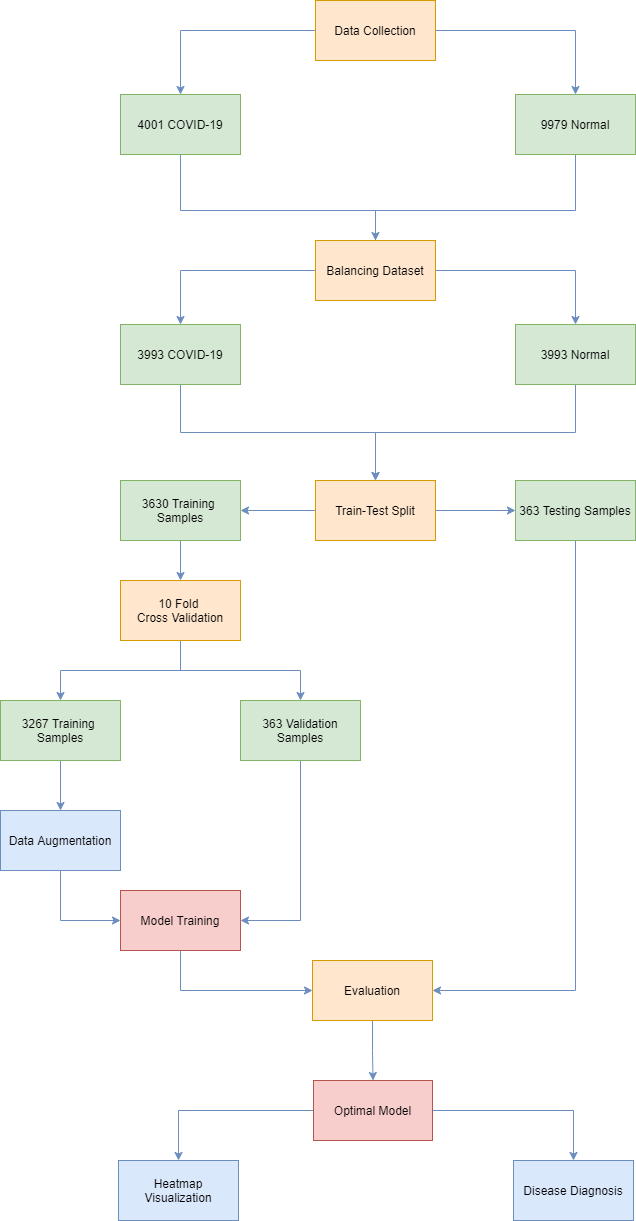
\includegraphics[width=13cm, height= 22.5cm]{Images/CT Workflow.png}

            %\decoRule
	\caption{\small CT Workflow Illustration}
	\label{fig:CT Illustration}
\end{figure}


\section{Web Interface}

Our Web Interface is a simple Diagnosis Portal allowing users to input X-ray or CT scans and retrieve real-time diagnosis and a heatmap highlighting critical regions. The front-end of the web application was built using Google's Flutter UI Toolkit. A Flask application was also deployed serving as backend containing Python scripts that retrieve diagnosis results. We have used an Ubuntu Virtual Machine offered by Microsoft Azure to deploy our Python Scripts and Web Application \footnote{Link to the Diagnosis Portal: \url{http://40.76.124.61/}}.

The Flask API provided an interface for the Flutter app, which takes the scan as input and returns diagnosis and heatmap. To ensure responsiveness of our Portal, we have utilized a custom responsive folder architecture \cite{agl2020}. We have uploaded a video demonstration of the Web Application, along with screenshots on OneDrive \footnote{Web Application Screenshots and Video Presentation can be found here: \url{https://heriotwatt-my.sharepoint.com/:f:/g/personal/agl2_hw_ac_uk/EgtAqrerqXZIhD3EPQJOJBsBJ3VTXhCZv_9pm_R01Bf8pA?e=z3mHHj}}. A subset of screenshots is displayed in Figure \ref{fig:portalScreenshots}.

\begin{figure}[H]
        \begin{subfigure}[b]{0.5\textwidth}
                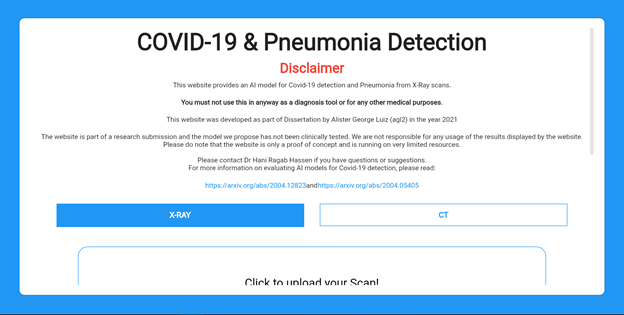
\includegraphics[width=\linewidth, height=4.3cm]{Images/Website Screenshot 1.png}
        \end{subfigure}%
        \begin{subfigure}[b]{0.5\textwidth}
                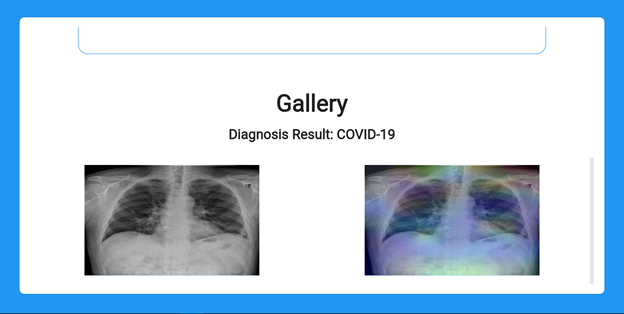
\includegraphics[width=\linewidth, height=4.3cm]{Images/Website Screenshot 2.png}
        \end{subfigure}%
        \vspace{0.8em}
        \begin{subfigure}[b]{0.5\textwidth}
                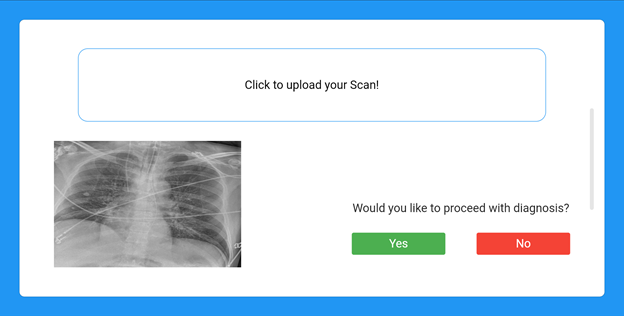
\includegraphics[width=\linewidth, height=4.3cm]{Images/Website Screenshot 5.png}
        \end{subfigure}%
        \begin{subfigure}[b]{0.5\textwidth}
                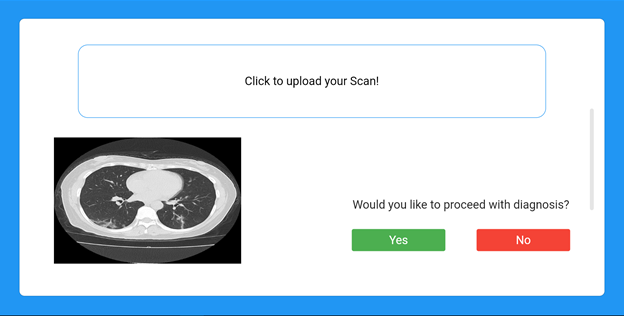
\includegraphics[width=\linewidth, height=4.3cm]{Images/Website Screenshot 7.png}
        \end{subfigure}%
        \vspace{0.8em}
        \begin{subfigure}[b]{0.5\textwidth}
                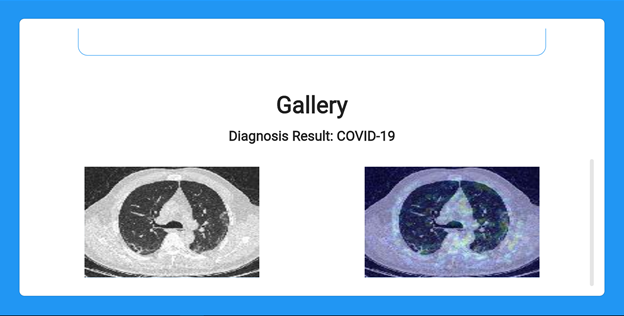
\includegraphics[width=\linewidth, height=4.3cm]{Images/Website Screenshot 3.png}
        \end{subfigure}%
        \begin{subfigure}[b]{0.5\textwidth}
                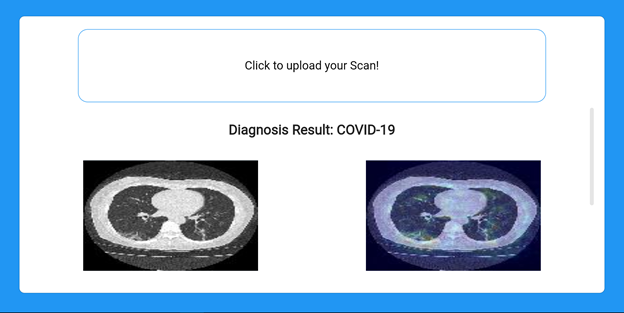
\includegraphics[width=\linewidth, height=4.3cm]{Images/Website Screenshot 8.png}
        \end{subfigure}%
        %\\\centering
        %\decoRule
        \caption{Diagnosis Portal Screenshots}\label{fig:portalScreenshots}
\end{figure}